\documentclass[12pt]{article}
\usepackage{setspace, graphicx, fullpage, amssymb, amsmath, epsfig, natbib, array, multirow, hyperref}
\usepackage{amsfonts, bm} 
\usepackage{dcolumn}
\usepackage{subfigure, float} 
\usepackage[margin=1in]{geometry} 
\usepackage{verbatim}
\usepackage{url}
\usepackage{enumerate}
\usepackage{morefloats}
\usepackage{caption}
\newcolumntype{d}[1]{D{.}{.}{#1}} 

\newcommand\fnote[1]{\captionsetup{font=small}\caption*{#1}}

\begin{document}

\section{Overview}

Last week we decided to do the following:

\begin{enumerate}
	\item Define which differences between tables are related to reelection and which of the non-election differences make sense
	
	\item Discuss the inclusion of the formal model
	
	\item Continue editing the paper
\end{enumerate}

\section{Differences Between House/Senate Results}

Those which concern the electoral connection:

\begin{itemize}
	
	\item Senate retirees are more responsive to party calls not significant for Democrats; no measure of this in current paper on House, mixed results in 2013 paper 
	
	\item Republicans with higher vote share in the Senate are significantly more likely to vote in favor of party call, insignificant (same sign) in House; positive significant for Senate minority, negative significant for House minority; negative significant for Dems in both chambers
	
\end{itemize}

\noindent
Things which are unsurprising/expected:

\begin{itemize}
	
	\item Most responsive extremists in House are Democrats/Minority Party and in Senate are Republicans/Minority Party (greater share of Southern Dems and ``Gingrich'' legislators could explain it)
	
	\item Party leader variable not significant for Senate Republicans, but positive coefficient for all
	
	\item Latino Senators' increased responsiveness not statistically significant in Senate for Democrats and minority party, is in House
	
	\item Power committee measure positive significant in all House subsets, negative insignificant in all Senate subsets
	
	\item In the Senate, responsiveness for committee chairs not increased as much as in House with some insignificant (positive and negative)
	
	\item Strength of prediction of baseline party vote rate differs by party in the House and is weaker than the Senate generally (though positive and significant for all)
	
\end{itemize}

\noindent
Things which are surprising/unexpected:

\begin{itemize}	
	
	\item Female legislators are more responsive to party calls in the Senate than the House 
	
	\item African American Republican Senators are much less likely to follow party calls, positive and insignificant relationship in House; significantly more likely for all in House to follow call, negative insignificant in Senate; significantly less likely in House majority to follow party call, positive significant in Senate
	
	\item Increasing seniority of Republicans in House significantly negatively impacts responsiveness, positive insignificant effect in Senate; Senate results closer to 2013 paper
	
	\item Being on a better committee in the House has a significant negative impact on party call responsiveness, has a positive impact that only achieves significance for minority party in Senate;
	Senate results closer to 2013 paper
	
\end{itemize}

\section{Formal Model}

The model as it exists now is entirely descriptive, rather than predictive, of what we are finding. In doing so, I fear that it will do more to raise questions than answer them as it stands. For instance, why should we expect in the Congress which members are up for reelection as a whole that members are taking constituents desires into account? Why do we think that they expect voters to remember a vote they made over a year before the date of reelection much more clearly than those they made a bit over two or three years before it, other than the fact that we have already found indications of this? 

Further, the model requires an assumption that voters are paying more attention to the party call votes than the noncall votes, but we have not investigated which bills in our data are party calls and which are not. This is something that could also be brought up with the arguments we develop in the main paper, and I worry that it would increase their chances of getting raised. Further, we don't have much of an explanation for which votes this should take effect on and why in the way that we have a measure for what constitutes a party call.

For these reasons, I would not want to include the formal model in the paper, though if desired we could include it in an appendix.

\pagebreak

\doublespacing
	
\section{Paper, Draft 5}

\begin{center}
	\large How Do Senators Vote When the Party Calls?
\end{center}

\begin{minipage}{15cm}
	\singlespacing
	\small \textit{Abstract}: In this paper, we replicate the findings of Minozzi \& Volden (2013) with some modifications of their methodology. We show that their hypotheses regarding party unity coming through the party working to unite more extreme (rather than more moderate) members holds not only in the House, but also the Senate. Further, we show the usefulness of separating votes by party influence as useful for demonstrating areas that affect the strength of party influence (but not ideology) by considering proximity to reelection in the Senate.
\end{minipage}

\subsection{Introduction}

Minozzi \& Volden (2013) developed the responsive extremists hypothesis to explain party unity on votes in the House of Representatives. This hypothesis holds that unity is typically a result of the party calling on members to support a position on bills which are coming up for a vote. Members' decisions to get in line with the party are based on their ideological extremism, which tracks with the benefits they get from the party brand, though they will at times have reasons to vote against the party. While pressuring of moderates occurs, it was held that such efforts were not as common or effective as the issuance of a party call. They tested this by sorting roll call votes into party influenced votes and party free votes and estimating the impact of member ideology on decision to respond to party influence.

This paper is written with the intention of replicating this paper and extending the units of analysis to include the Senate and the period of analysis to Congresses 93-112. Party calls and member responsiveness to them are well-suited to drawing inferences on member behavior. Given their high party unity, these votes are likely to attract larger amounts of attention than other votes which occur in a Congress. However, they are also likely to be more important to the party and voting against the party on them could be damaging to the party's agenda. We believe that party calls are a beneficial metric for considering member behavior since they separate the role of party and ideology, as is necessary (Krehbiel, 1993; Lee, 2009). This separation of influence allows for much more thorough considerations of member behavior than do considerations of behavior of all votes as though decisions on them are equivalent.

We know that members can reap benefits from parties (Lee, 2009) but that members who are perceived to be holding the interests of the party above those of their district are electorally punished (Canes-Wrone, Brady \& Cogan, 2002; Carson et al., 2010). Members' primary goal is to be reelected, since other goals cannot be achieved without this (Mayhew, 1974). Unsurprisingly, the behavior of Senators takes their district into much greater account when they approach reelection (Levitt, 1996). We view it as likely that member voting behavior would change in regard to party calls, but not other votes, because they can more clearly show on these votes that they are willing to take principled stands against their party. Such a change would not be expected in noncall votes, since members are already voting on these based primarily on personal preferences, something voters are likely to be pleased with.

In the following section we show the results of our replication with a set of tests designed to further explore and explain Senator behavior as reelection approaches following it. Our extensions allow us to test the responsive extremists hypothesis in both chambers, with consideration of more recent Congresses which both chambers are held to have become more extreme. Additionally, the inclusion of the Senate allows for tests to be conducted based on proximity to reelection. We find that the responsive extremist hypothesis developed by Minozzi \& Volden holds in this expanded set of cases. Further, we find that Senators will vote along with the party on a couple fewer party calls in Congresses they are up for reelection than they would otherwise be expected to.

\subsection{Replication with Extension}

In this section we provide the results of the replication with extension to the Senate and into Congresses 93-112. This analysis involved the use of an algorithm which sorted votes into party calls and party free votes based on whether vote choice was significantly predicted by party status. Member ideology is based on the party free votes and the ideal points calculated by one iteration is used to also predict vote choice in the next. Our model is a modified version of the one described in Minozzi \& Volden (2013). Ideological extremism is member party free ideal point, with sign reversed for Democrats (so that it is higher for members of each party as they become more extreme).\footnote{A more thorough overview of the methodology is detailed in an appendix.}

We find that party calls are more present in the House, but that they appear in the Senate as well. Additionally, we find that in both chambers their incidence has been on an upward trend during our period of analysis. We believe this trend merits further investigation, but initially take it as evidence of increased partisanship in recent decades, in line with others' findings (Lee, 2009; Theriault, 2013; Smith, 2014).


\begin{figure}[H]
	\centering
	\caption{Party Calls as a Percentage of Votes, Congresses 93-112}
	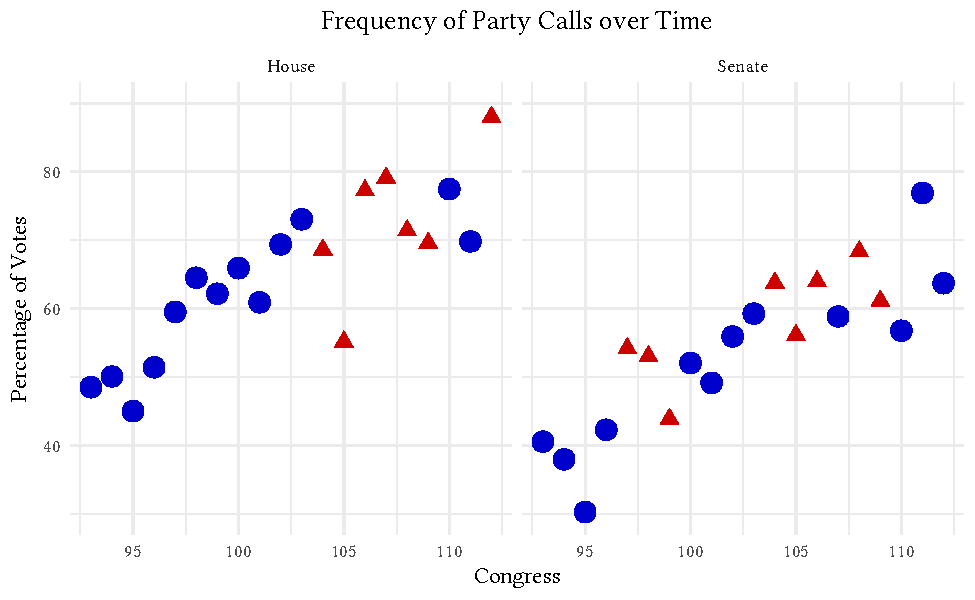
\includegraphics[width = \textwidth]{C:/Users/Ethan/Documents/GitHub/partycalls/plots/party_call_percent_both.pdf}
	\fnote{\textit{Note}: Blue circles denote Democrat majority Congresses while Red triangles denote Republican majority Congresses. Trend lines fit with OLS.}
\end{figure}

Regression analysis, with all member pooled or separated by party and majority status broadly show the responsive extremists hypothesis to hold. In both chambers we find that increased ideological extremism leads to increased responsiveness on party call votes. We find that Southern Democrats are less responsive to the party than are other Democrats, unsurprising since they have typically been near the chamber median. We also note that the power committee variable we constructed for the Senate (based on membership in a top 4 committee) carries little predictive power, either in terms of substantive power or statistical significance. This is not entirely unexpected, since this is a variable we included less because we believed it had meaning to Senators and more for model comparability. We also note that in both chambers increased same party presidential vote share within one's constituency makes Democrats more likely to respond to a party call but reduces the chances of a Republican doing so.

\begin{table}[H]
	\begin{center}
		\singlespacing
		\small
		\caption{House Responsiveness to Party Calls}
		%\footnotesize
		\begin{tabular}{l c c c c c }
			\hline
			& All & Democrats & Republicans & Majority & Minority \\
			\hline
			Ideological Extremism & $7.728^{***}$  & $8.320^{***}$  & $5.752^{***}$  & $6.605^{***}$  & $8.572^{***}$  \\
			& $(0.129)$      & $(0.168)$      & $(0.205)$      & $(0.155)$      & $(0.201)$      \\
			Baseline Rate of Voting with Party              & $0.569^{***}$  & $0.636^{***}$  & $0.397^{***}$  & $0.528^{***}$  & $0.599^{***}$  \\
			& $(0.012)$      & $(0.015)$      & $(0.020)$      & $(0.014)$      & $(0.019)$      \\
			Vote Share            & $-0.015$       & $-0.051^{***}$ & $0.026$        & $-0.119^{***}$ & $-0.050^{***}$ \\
			& $(0.009)$      & $(0.009)$      & $(0.016)$      & $(0.010)$      & $(0.015)$      \\
			Pres Vote Share      & $0.034^{***}$  & $0.096^{***}$  & $-0.098^{***}$ & $0.208^{***}$  & $0.164^{***}$  \\
			& $(0.009)$      & $(0.011)$      & $(0.019)$      & $(0.011)$      & $(0.017)$      \\
			South                  & $-0.928^{***}$ & $-2.496^{***}$ & $3.554^{***}$  & $-1.687^{***}$ & $-0.575$       \\
			& $(0.203)$      & $(0.274)$      & $(0.327)$      & $(0.242)$      & $(0.311)$      \\
			Female                 & $1.226^{***}$  & $0.682^{*}$    & $-0.080$       & $0.137$        & $2.170^{***}$  \\
			& $(0.318)$      & $(0.347)$      & $(0.570)$      & $(0.394)$      & $(0.442)$      \\
			African American                   & $1.915^{***}$  & $-0.270$       & $5.212$        & $-2.637^{***}$ & $3.149^{***}$  \\
			& $(0.421)$      & $(0.433)$      & $(2.986)$      & $(0.524)$      & $(0.603)$      \\
			Latino                 & $3.236^{***}$  & $1.881^{***}$  & $2.178$        & $2.706^{***}$  & $3.248^{***}$  \\
			& $(0.500)$      & $(0.505)$      & $(1.150)$      & $(0.612)$      & $(0.701)$      \\
			Seniority              & $-0.050$       & $0.059$        & $-0.337^{***}$ & $0.039$        & $-0.007$       \\
			& $(0.028)$      & $(0.031)$      & $(0.050)$      & $(0.034)$      & $(0.041)$      \\
			Freshman               & $0.601^{*}$    & $-0.057$       & $0.914^{*}$    & $0.197$        & $-0.358$       \\
			& $(0.288)$      & $(0.343)$      & $(0.450)$      & $(0.334)$      & $(0.435)$      \\
			Best Committee          & $-0.162^{***}$ & $-0.037^{*}$   & $-0.233^{***}$ & $-0.166^{***}$ & $-0.171^{***}$ \\
			& $(0.015)$      & $(0.018)$      & $(0.025)$      & $(0.018)$      & $(0.022)$      \\
			Party leader                 & $1.800^{***}$  & $1.926^{**}$   & $2.838^{***}$  & $2.421^{***}$  & $1.863^{**}$   \\
			& $(0.495)$      & $(0.593)$      & $(0.761)$      & $(0.633)$      & $(0.662)$      \\
			Power Committee                  & $2.773^{***}$  & $1.902^{***}$  & $2.814^{***}$  & $3.005^{***}$  & $1.143^{**}$   \\
			& $(0.233)$      & $(0.274)$      & $(0.371)$      & $(0.265)$      & $(0.361)$      \\
			Committee Chair                  & $5.008^{***}$  & $2.430^{***}$  & $9.714^{***}$  & $1.821^{***}$  &                \\
			& $(0.454)$      & $(0.497)$      & $(0.798)$      & $(0.439)$      &                \\
			(Intercept)            & $31.980^{***}$ & $24.690^{***}$ & $53.184^{***}$ & $36.980^{***}$ & $20.097^{***}$ \\
			& $(1.269)$      & $(1.580)$      & $(2.159)$      & $(1.484)$      & $(2.014)$      \\
			\hline
			R$^2$                  & 0.460          & 0.635          & 0.295          & 0.573          & 0.465          \\
			Adj. R$^2$             & 0.459          & 0.634          & 0.292          & 0.572          & 0.464          \\
			Num. obs.              & 8785           & 4886           & 3899           & 5043           & 3742           \\
			RMSE                   & 8.486          & 7.395          & 8.910          & 7.540          & 8.132          \\
			\hline
			\multicolumn{6}{l}{\scriptsize{$^{***}p<0.001$, $^{**}p<0.01$, $^*p<0.05$}}
		\end{tabular}
	\fnote{Results are produced by OLS regressions for all Democrats and Republicans as well as all members of the Majority and Minority party in Congresses 93-112 in the House of Representatives. Most variables provided by the Legislative Effectiveness Project.}
	\end{center}
\end{table}

\begin{table}[H]
	\begin{center}
		\singlespacing
		\small
		\caption{Senate Responsiveness to Party Calls}
		%\footnotesize
		\begin{tabular}{l c c c c c }
			\hline
			& All & Democrats & Republicans & Majority & Minority \\
			\hline
			Ideological Extremism & $6.239^{***}$  & $3.136^{***}$ & $7.792^{***}$  & $4.708^{***}$  & $7.949^{***}$ \\
			& $(0.252)$      & $(0.409)$     & $(0.357)$      & $(0.315)$      & $(0.400)$     \\
			Committee Chair                  & $2.105^{***}$  & $0.852$       & $3.626^{***}$  & $-0.017$       &               \\
			& $(0.452)$      & $(0.543)$     & $(0.700)$      & $(0.517)$      &               \\
			Baseline Rate of Voting with Party              & $0.737^{***}$  & $0.759^{***}$ & $0.742^{***}$  & $0.702^{***}$  & $0.702^{***}$ \\
			& $(0.021)$      & $(0.030)$     & $(0.031)$      & $(0.025)$      & $(0.035)$     \\
			Presidential Vote Share      & $0.097^{***}$  & $0.234^{***}$ & $-0.134^{***}$ & $0.182^{***}$  & $0.006$       \\
			& $(0.018)$      & $(0.024)$     & $(0.031)$      & $(0.020)$      & $(0.032)$     \\
			South                  & $0.613$        & $-1.690^{**}$ & $0.872$        & $0.054$        & $1.085$       \\
			& $(0.362)$      & $(0.557)$     & $(0.578)$      & $(0.427)$      & $(0.622)$     \\
			Power Committee       & $-0.684$       & $-0.855$      & $-0.325$       & $-0.052$       & $-1.468$      \\
			& $(0.620)$      & $(0.772)$     & $(0.924)$      & $(0.719)$      & $(1.064)$     \\
			Vote Share            & $0.029$        & $-0.053^{*}$  & $0.149^{***}$  & $-0.012$       & $0.076^{*}$   \\
			& $(0.018)$      & $(0.022)$     & $(0.028)$      & $(0.021)$      & $(0.030)$     \\
			Female                 & $2.041^{**}$   & $1.690^{*}$   & $0.451$        & $0.532$        & $4.256^{***}$ \\
			& $(0.638)$      & $(0.730)$     & $(1.132)$      & $(0.758)$      & $(1.113)$     \\
			African American                   & $-4.769$       & $-1.164$      & $-10.789^{*}$  & $1.531$        & $-5.519$      \\
			& $(2.486)$      & $(2.789)$     & $(4.278)$      & $(4.184)$      & $(3.219)$     \\
			Latino                 & $5.717^{**}$   & $1.814$       & $7.264^{**}$   & $4.781^{*}$    & $6.253$       \\
			& $(1.816)$      & $(2.198)$     & $(2.779)$      & $(1.878)$      & $(3.506)$     \\
			Up For Reelection    & $-0.908^{*}$   & $-0.630$      & $-1.436^{**}$  & $-0.951^{*}$   & $-1.204^{*}$  \\
			& $(0.353)$      & $(0.426)$     & $(0.538)$      & $(0.411)$      & $(0.603)$     \\
			Seniority              & $0.002$        & $0.041$       & $-0.024$       & $0.077$        & $0.118$       \\
			& $(0.044)$      & $(0.052)$     & $(0.072)$      & $(0.060)$      & $(0.070)$     \\
			Freshman               & $0.859$        & $0.769$       & $0.358$        & $0.600$        & $0.996$       \\
			& $(0.566)$      & $(0.708)$     & $(0.842)$      & $(0.631)$      & $(1.032)$     \\
			Retiree                & $2.103^{**}$   & $1.599$       & $2.290^{*}$    & $1.816^{*}$    & $2.575^{*}$   \\
			& $(0.693)$      & $(0.897)$     & $(0.997)$      & $(0.850)$      & $(1.110)$     \\
			Best Committee        & $0.163$        & $0.237$       & $0.008$        & $0.027$        & $0.373^{*}$   \\
			& $(0.101)$      & $(0.124)$     & $(0.154)$      & $(0.118)$      & $(0.174)$     \\
			Party Leader                 & $1.604^{**}$   & $2.218^{**}$  & $0.910$        & $1.441^{*}$    & $1.940^{*}$   \\
			& $(0.539)$      & $(0.712)$     & $(0.776)$      & $(0.661)$      & $(0.899)$     \\
			(Intercept)            & $11.611^{***}$ & $9.447^{**}$  & $18.182^{***}$ & $16.365^{***}$ & $10.799^{**}$ \\
			& $(2.274)$      & $(2.906)$     & $(3.489)$      & $(2.644)$      & $(4.009)$     \\
			\hline
			R$^2$                  & 0.632          & 0.689         & 0.641          & 0.684          & 0.615         \\
			Adj. R$^2$             & 0.629          & 0.684         & 0.635          & 0.679          & 0.608         \\
			Num. obs.              & 1993           & 1042          & 951            & 1052           & 843           \\
			RMSE                   & 6.967          & 6.118         & 7.255          & 5.865          & 7.749         \\
			\hline
			\multicolumn{6}{l}{\scriptsize{$^{***}p<0.001$, $^{**}p<0.01$, $^*p<0.05$}}
		\end{tabular}
	\fnote{Results are produced by OLS regressions for all Democrats and Republicans as well as all members of the Majority and Minority party in Congresses 93-112 in the House of Representatives. Most variables provided by the Legislative Effectiveness Project, with supplementary data for committees from Charles Stewart's Congressional data and retirement data from the Congressional Bioguides.}
	\end{center}
\end{table}

In Table 2, we see strong evidence of the predicted differences between members up for reelection and others. Across all subgroups this coefficient is negative, and the effect viewed is negative for all other than Democrats. Finally, we show coefficient plots for ideological extremism in the House and Senate. 

\begin{figure}[H]
	\centering
	\caption{House Ideological Extremism Coefficient Plot}
	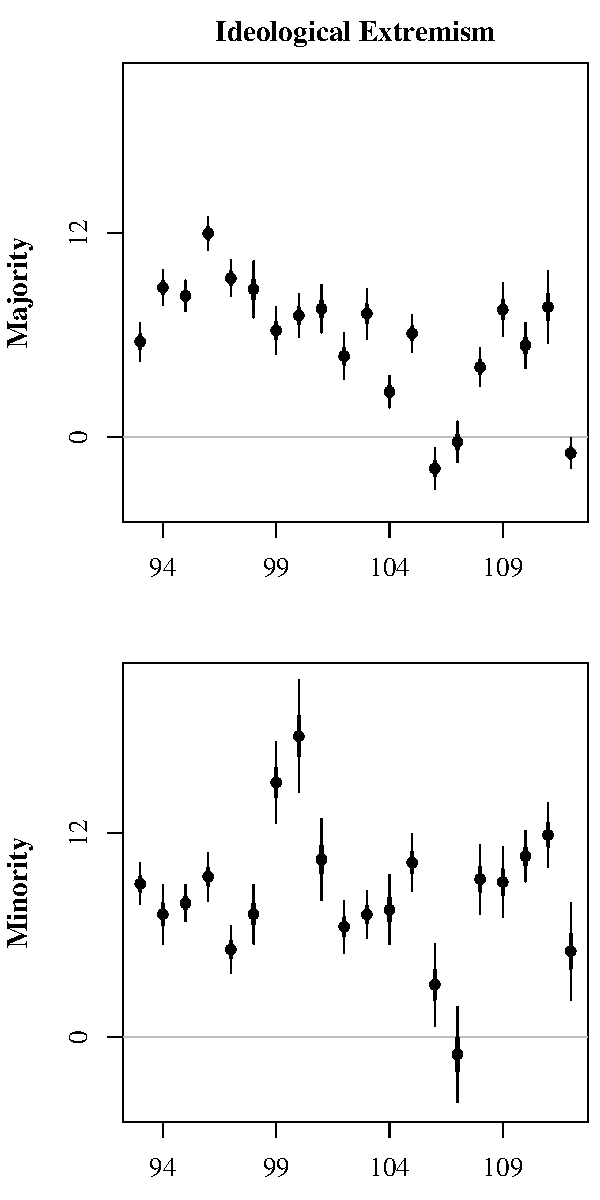
\includegraphics[width = 7cm]{C:/Users/Ethan/Documents/GitHub/partycalls/plots/who-heeds-figure2-replication_lm.pdf}
	\fnote{This coefficient plot is produced by the same formula shown in the House regression table with results decomposed by individual Congresses for the Majority and Minority parties. Coefficients shown are for the effect of ideological extremism on party free votes in relation to party call votes. 50\% and 95\% confidence intervals are shown from the points.}
\end{figure}

\begin{figure}[H]
	\centering
	\caption{Senate Ideological Extremism Coefficient Plot}
	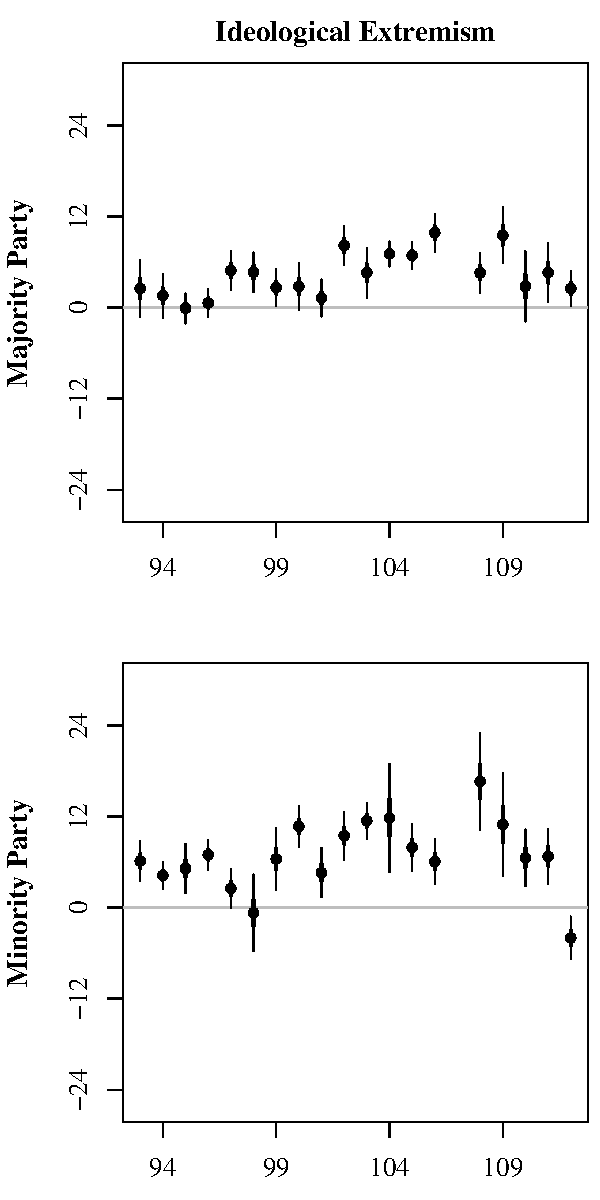
\includegraphics[width = 7cm]{C:/Users/Ethan/Documents/GitHub/partycalls/plots/senate-figure2-lm.pdf}
	\fnote{This coefficient plot is produced by the same formula shown in the Senate regression table with results decomposed by individual Congresses for the Majority and Minority parties. Coefficients shown are for the effect of ideological extremism on party free votes in relation to party call votes. 50\% and 95\% confidence intervals are shown from the points.}
\end{figure}

We note that though ideological extremism is a significant predictor in the regression analyses which rely on all Congresses, it fails to achieve significance for all Congresses taken separately in the Senate. We are unsurprised by this since each party in a given Senate has far fewer members than does a party in the House. So, we remain confident that party calls are present in both chambers and behave in broadly similar ways. Having established this, we turn to the case of reelection in the Senate, which we see as a useful area to consider how members balance ideology and party preferences. The use of party call responsiveness provides results in line with our expectations for member behavior when approaching reelection.

\subsection{Reelection in the Senate}

In this section we test specifically for differences in member responsiveness by proximity to reelection. In order to do this, we estimate models which rely on same-state Senator pairs when one of them is up for reelection at the end of the Congress. These pairings are ideal since an expectation is that members will respond according to their voters and same-state Senators are elected by the same voters. So, we are confident in assuming that these pairs will change their behavior in comparable ways as reelection approaches. 

The fact that same-state Senators are not up for reelection at the same time allows us to estimate a generalization of a difference-in-differences design on pairs in Congresses which one is up for reelection. We use this to compare member responsiveness to the party on party calls, the baseline rate of voting with the party, and the difference between these two quantities between the member up for reelection and the member in the beginning or middle of their term. For each of these, a placebo test with randomly assigned treatment is also shown.\footnote{Reported 50\% and 95\% confidence intervals are developed by a bootstrap sample. More details about this and other areas of the methodology can be found in an appendix.} Cases which have more than two Senators from a state during a single Congress (due to deaths and retirements) are dropped from the analysis.

\begin{figure}[H]
	\centering
	\caption{Senate Rate of Voting With Party by Vote Type}
	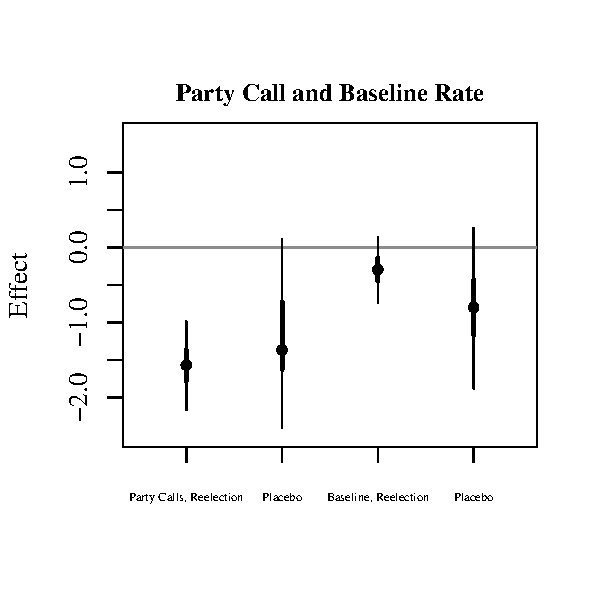
\includegraphics[width = 10cm]{C:/Users/Ethan/Documents/GitHub/partycalls/plots/senate-diff-in-diff-coeff-separate.pdf}
	\fnote{\textit{Note}: This coefficient plot is produced by a paired differences model which uses same-state Senators as a natural pairing. Differences between member responsiveness to party calls are shown by the first two points with the second set representing differences in baseline rate of voting with the party. The first and third columns use proximity to reelection as a treatment which are compared in columns 2 and 4 with a placebo treatment of the Senator with higher seniority in Congresses which neither are up for reelection as a comparison. 50\% and 95\% confidence intervals are shown.}
\end{figure}

\begin{figure}[H]
	\centering
	\caption{Senate Rate of Voting With Party by Vote Type}
	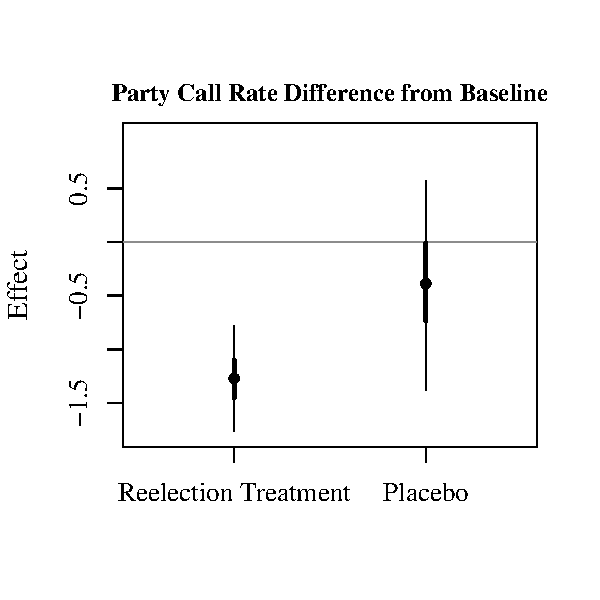
\includegraphics[width = 10cm]{C:/Users/Ethan/Documents/GitHub/partycalls/plots/senate-diff-in-diff-coeff.pdf}
	\fnote{\textit{Note}: This coefficient plot is produced by a paired difference-in-differences model which considers the difference between same-state Senator responsiveness to party calls from their baseline rate of voting with the party. The first column uses proximity to reelection as a treatment while the second uses higher seniority in Congresses which neither is up for reelection as a placebo treatment. 50\% and 95\% confidence intervals are shown.}
\end{figure}

The results of these tests clearly show that member responsiveness to party calls declines, on average, about 1.5\% when they are up for reelection.\footnote{Since the average number of party calls in a Congress during the time we analyze is approximately 365, this means that a Senate party can generally expect to count on members up for reelection for a little over 5 votes against the party's position on party call votes.} This slight change in posture would be enough to allow them to point to multiple additional instances in which they went against the party to their voters and to do so without greatly hindering the party's goals. Member voting behavior on other votes does not exhibit this relationship, likely due to them not being perceived as providing as clear of a signal to voters. Thus, we conclude that member proximity to reelection leads members to place greater weight on seeming different from the party in order to appease voters at key moments.

Given that members are less responsive to party calls when they are approaching reelection, it merits further investigation why we see more party calls in the House than in the Senate, since House members are always up for reelection at the end of a term. 



\subsection{Conclusion}

In this paper, we tested if members respond to party calls in the Senate as they do in the House, using analyses based on those of Minozzi \& Volden (2013). This allowed us not only to confirm their results, but also to show the potential advantages of party calls as a method for viewing member behavior related to ideology and partisanship. We showed that reelection modifies member behavior on roll call votes which party is a factor in, but not those which are based primarily on ideology. This is in line with expectations of members working to consider voter preferences more highly as reelection becomes more proximate, though it expands on previous studies by highlighting specific conditions under which member behavior changes and others which it remains constant.

\pagebreak

\section{Appendices}

\subsection{Appendix A: Detailing the New Sorting Algorithm}

As was done by Minozzi \& Volden (2013) we develop an algorithm to sort votes based on the degree to whether vote choice can be significantly predicted by party or caucus membership after ideology is accounted for. In this algorithm, member ideology in one iteration is calculated on the votes which were not party calls in the previous iteration since party is accounting for some of the weight in decision on the other set. Ideology for the first iteration is calculated on votes which have more than 65\% or less than 35\% of members of the chamber voting on the same side. The algorithm has a 15 iteration burn in period for each Congress. Once this has concluded, the algorithm continues either until the number of votes switched has hit a minimum and begun to climb or until there are fewer than 5 votes which switch between iterations. Once these conditions are met, it continues for 15 additional iterations, the last 5 of which are used to identify party calls and non calls. Any votes which switched between party calls and non party calls during the final 5 iterations are dropped from our analyses.

One of the key changes was the use of the \verb|binIRT()| R function from the \verb|emIRT|in order to calculate members' party free ideology, replacing \verb|ideal()| which was used by Minozzi \& Volden. The \verb|binIRT()| function was developed by Imai, Lo \& Olmsted in order to produce estimates analagous to those of \verb|ideal()| with reduced computational taxation. We find both of these aims to be met.

We find that the party call is not merely produced by a tradeoff of party and ideology explaining different votes; they are on the same side approximately two-thirds of the time in the House and three-fifths of the time in the Senate.

% latex table generated in R 3.3.2 by xtable 1.8-2 package
% Thu Feb 23 17:39:42 2017
\begin{table}[H]
	\centering
	\singlespacing
	\caption{House Sorting Algorithm Coefficient Signs}
	\begin{tabular}{rrr}
		\hline
		& ($-$) Ideal & (+) Ideal \\ 
		\hline
		(-) Party & 0.38 & 0.15 \\ 
		(+) Party & 0.17 & 0.30 \\ 
		\hline
	\end{tabular}
\fnote{The party variable used in this analysis is an indicator for status as a Republican, and thus would be expected to correlate positively with ideal points.}
\end{table}

% latex table generated in R 3.3.2 by xtable 1.8-2 package
% Thu Feb 23 17:23:31 2017
\begin{table}[H]
	\centering
	\singlespacing
	\caption{Senate Sorting Algorithm Coefficient Signs}
	\begin{tabular}{rrr}
		\hline
		& ($-$) Ideal & (+) Ideal \\ 
		\hline
		($-$) Party & 0.33 & 0.16 \\ 
		(+) Party & 0.23 & 0.28 \\ 
		\hline
	\end{tabular}
\fnote{The party variable used in this analysis is an indicator for status as a Republican, and thus would be expected to correlate positively with ideal points.}
\end{table}

We found that the lowered number of both members and bills in the Senate required a few changes to the vote sorting method, however. Since $p$-values will necessarily be lower with fewer observations, we had to change the threshold for party calls to $p <$ 0.05 (from $p <$ 0.01). Next, since the ideal point algorithm uses a logistic regression, problems arose in vote sorting when we also tried to use another to sort vote type with this in the Senate. Neither change leads the sorting in the House to differ for the most part. We find that the sorting of close and lopsided votes by this method to be in line with Minozzi \& Volden's findings.

% latex table generated in R 3.3.2 by xtable 1.8-2 package
% Mon Mar 20 13:02:44 2017
\begin{table}[H]
	\centering
	\singlespacing
	\caption{House Vote Coding for Close and Lopsided Votes} 
	\begin{tabular}{lrr}
		\hline
		& Party Call & Noncall \\ 
		\hline
		Lopsided & 4245 & 6123 \\ 
		Close & 9308 & 1090 \\ 
		\hline
	\end{tabular}
\fnote{The threshold for a vote to be lopsided was 65\% of members (or conversely, 35\%) voting on the same side of a roll call vote.}
\end{table}

% latex table generated in R 3.3.2 by xtable 1.8-2 package
% Mon Mar 20 13:04:18 2017
\begin{table}[H]
	\centering
	\singlespacing
	\caption{Senate Vote Coding for Close and Lopsided Votes} 
	\begin{tabular}{lrr}
		\hline
		& Party Call & Noncall \\ 
		\hline
		Lopsided & 2063 & 4876 \\ 
		Close & 5233 & 1851 \\ 
		\hline
	\end{tabular}
\fnote{The threshold for a vote to be lopsided was 65\% of members (or conversely, 35\%) voting on the same side of a roll call vote.}
\end{table}













\subsection{Appendix B: Methodology for Senate Reelection Section}

In order to better test the role of reelection we use same-state senators as a natural pairing. These results were shown in figures 2 and 3 in the paper. The analyses we performed on these pairs were generalizations of the difference in differences design, in which the member not up for reelection had their response rate subtracted from that of the member who was up for reelection. Figure 2 showed the differences by vote type and figure 3 showed the change between vote types between these pairs. For each of these, we also performed analyses on Congresses which neither was up for reelection as a placebo test, with the ``treatment'' being based on which member was more senior. Here we show the results in tables, with breakdowns by seat pair type.

% latex table generated in R 3.3.2 by xtable 1.8-2 package
% Mon Mar 27 22:28:47 2017
\begin{table}[H]
	\centering
	\singlespacing
	\caption{Reelection and Response to Party Calls, Difference in Differences} 
	\begin{tabular}{llrrr}
		\hline
		Test & DV & Estimate & Lower Bound & Upper Bound \\ 
		\hline
		Effect & pirate100 & -1.569 & -2.139 & -1.001 \\ 
		Placebo & pirate100 & -0.331 & -1.281 & 1.259 \\ 
		Effect & pfrate100 & -0.297 & -0.798 & 0.126 \\ 
		Placebo & pfrate100 & -0.644 & -1.074 & 1.143 \\ 
		\hline
	\end{tabular}
\end{table}

% latex table generated in R 3.3.2 by xtable 1.8-2 package
% Mon Mar 27 22:28:47 2017
\begin{table}[H]
	\centering
	\singlespacing
	\caption{Diff in Diff, Subgroup Condition, Party Influenced Rate} 
	\begin{tabular}{llr}
		\hline
		Test & DV & Estimate \\ 
		\hline
		2 Maj Dems Effect & pirate100 & 0.0708958 \\ 
		2 Maj Dems Placebo & pirate100 & -0.4769119 \\ 
		2 Min Dems Effect & pirate100 & -1.8733904 \\ 
		2 Min Dems Placebo & pirate100 & -1.2633351 \\ 
		2 Maj Reps Effect & pirate100 & -1.1307379 \\ 
		2 Maj Reps Placebo & pirate100 & -2.2707921 \\ 
		2 Min Reps Effect & pirate100 & 0.3990873 \\ 
		2 Min Reps Placebo & pirate100 & -1.9947329 \\ 
		Split, Maj Dem, Dem Effect & pirate100 & 3.8789004 \\ 
		Split, Maj Dem, Dem Placebo & pirate100 & 0.7159106 \\ 
		Split, Maj Dem, Rep Effect & pirate100 & -8.6767819 \\ 
		Split, Maj Dem, Rep Placebo & pirate100 & -1.0729345 \\ 
		Split, Maj Rep, Dem Effect & pirate100 & -8.0169523 \\ 
		Split, Maj Rep, Dem Placebo & pirate100 & -2.1276690 \\ 
		Split, Maj Rep, Rep Effect & pirate100 & 0.0096892 \\ 
		Split, Maj Rep, Rep Placebo & pirate100 & 0.0232939 \\ 
		\hline
	\end{tabular}
\end{table}

% latex table generated in R 3.3.2 by xtable 1.8-2 package
% Sun Mar 26 19:10:24 2017
\begin{table}[H]
	\centering
	\singlespacing
	\caption{Reelection and Response to Party Calls, Difference in Differences} 
	\begin{tabular}{llrrr}
		\hline
		test & DV & Estimate & Lower Bound & Upper Bound \\ 
		\hline
		Effect & pirate100 - pfrate100 & -1.272 & -1.775 & -0.794 \\ 
		Placebo & pirate100 - pfrate100 & -0.292 & -0.904 & 0.935 \\ 
		\hline
	\end{tabular}
\end{table}

% latex table generated in R 3.3.2 by xtable 1.8-2 package
% Sun Mar 26 19:10:27 2017
\begin{table}[H]
	\centering
	\caption{Diff in Diff, Subgroup Condition, Party Influenced Rate} 
	\begin{tabular}{llr}
		\hline
		Test & DV & Estimate \\ 
		\hline
		2 Maj Dems Effect & pirate100 - pfrate100 & -0.1191943 \\ 
		2 Maj Dems Placebo & pirate100 - pfrate100 & 0.5657017 \\ 
		2 Min Dems Effect & pirate100 - pfrate100 & -1.8253378 \\ 
		2 Min Dems Placebo & pirate100 - pfrate100 & -0.4463733 \\ 
		2 Maj Reps Effect & pirate100 - pfrate100 & -2.2112471 \\ 
		2 Maj Reps Placebo & pirate100 - pfrate100 & -0.1749949 \\ 
		2 Min Reps Effect & pirate100 - pfrate100 & 0.7774782 \\ 
		2 Min Reps Placebo & pirate100 - pfrate100 & -0.4516436 \\ 
		Split, Maj Dem, Dem Effect & pirate100 - pfrate100 & -0.8756821 \\ 
		Split, Maj Dem, Dem Placebo & pirate100 - pfrate100 & -1.8454871 \\ 
		Split, Maj Dem, Rep Effect & pirate100 - pfrate100 & -1.4582552 \\ 
		Split, Maj Dem, Rep Placebo & pirate100 - pfrate100 & 0.0117995 \\ 
		Split, Maj Rep, Dem Effect & pirate100 - pfrate100 & -7.1166813 \\ 
		Split, Maj Rep, Dem Placebo & pirate100 - pfrate100 & -3.4630959 \\ 
		Split, Maj Rep, Rep Effect & pirate100 - pfrate100 & 0.3772151 \\ 
		Split, Maj Rep, Rep Placebo & pirate100 - pfrate100 & 0.2964502 \\ 
		\hline
	\end{tabular}
\end{table}

As a further test, not shown in the paper, we estimated the effect of reelection and other variables with a fixed effects model. This produces substantively similar effects to those reported in the main paper. Most notable to us is that the effect produced by being up for reelection is in line with findings shown in the main paper.

\begin{table}[H]
	\begin{center}
		\caption{Senate Fixed Effects Models, Party Call Response Rate}
		\begin{tabular}{l c c c c }
			\hline
			& Democrats & Republicans & Majority & Minority \\
			\hline
			Ideological Extremism  & $2.88^{***}$ & $4.00^{***}$  & $1.80^{**}$   & $3.93^{***}$ \\
			& $(0.69)$     & $(0.75)$      & $(0.64)$      & $(0.97)$     \\
			Baseline Rate of Voting with Party               & $0.37^{***}$ & $0.25^{***}$  & $0.37^{***}$  & $0.18^{*}$   \\
			& $(0.05)$     & $(0.05)$      & $(0.05)$      & $(0.07)$     \\
			Up For Reelection     & $-0.55^{*}$  & $-1.55^{***}$ & $-1.02^{***}$ & $-1.04^{**}$ \\
			& $(0.27)$     & $(0.34)$      & $(0.28)$      & $(0.37)$     \\
			Vote Share             & $0.03$       & $-0.05$       & $0.02$        & $-0.02$      \\
			& $(0.02)$     & $(0.03)$      & $(0.03)$      & $(0.04)$     \\
			Presidential Vote Share       & $0.27^{***}$ & $0.09$        & $0.31^{***}$  & $0.14^{*}$   \\
			& $(0.04)$     & $(0.05)$      & $(0.06)$      & $(0.06)$     \\
			Freshman                & $0.71$       & $0.98^{*}$    & $0.77$        & $0.78$       \\
			& $(0.48)$     & $(0.46)$      & $(0.46)$      & $(0.76)$     \\
			Retiree                 & $0.25$       & $0.88$        & $0.36$        & $0.75$       \\
			& $(0.83)$     & $(0.83)$      & $(0.99)$      & $(0.91)$     \\
			Best Committee         & $0.14$       & $0.11$        & $0.29$        & $0.36^{*}$   \\
			& $(0.12)$     & $(0.16)$      & $(0.15)$      & $(0.18)$     \\
			Power Committee        & $-0.48$      & $-0.22$       & $-1.26$       & $-0.45$      \\
			& $(0.70)$     & $(0.98)$      & $(0.89)$      & $(1.01)$     \\
			Leader                  & $0.87$       & $1.46^{*}$    & $1.39$        & $1.31$       \\
			& $(0.47)$     & $(0.62)$      & $(0.78)$      & $(0.80)$     \\
			Committee Chair                   & $0.38$       & $0.65$        & $-0.57$       &              \\
			& $(0.64)$     & $(0.71)$      & $(0.56)$      &              \\
			\hline
			Num. obs.               & 1042         & 951           & 1052          & 843          \\
			R$^2$      & 0.89         & 0.91          & 0.92          & 0.94         \\
			Adj. R$^2$ & 0.87         & 0.88          & 0.89          & 0.91         \\
			\hline
			\multicolumn{5}{l}{\scriptsize{$^{***}p<0.001$, $^{**}p<0.01$, $^*p<0.05$}}
		\end{tabular}
	\end{center}
\end{table}

\subsection{Appendix C: Other Tables and Figures from Replication}

In Minozzi \& Volden (2013), the regression table produced shows results in Congresses 97, 102, and 107 divided by party. Here, we produce the results from our analyses in the House of these chambers for ideological extremism\footnote{Since distance from floor median was not calculated for or used by any of our analyses, we do not replicate any of their analyses which use it}.

\begin{table}
	\begin{center}
		\caption{Replication of Minozzi \& Volden (2013), Table 3}
		\begin{tabular}{l c c c c c c }
			\hline
			& \multicolumn{3}{c}{Democrats} & \multicolumn{3}{c}{Republicans} \\
			\cline{2-7}
			& 97th & 102nd & 107th & 97th & 102nd & 107th \\
			\hline
			Ideological Extremism & $9.27^{***}$  & $5.07^{***}$  & $-1.11$      & $5.21^{***}$ & $6.78^{***}$  & $-0.20$       \\
			& $(0.53)$      & $(0.69)$      & $(1.50)$     & $(0.71)$     & $(0.76)$      & $(0.61)$      \\
			Baseline Rate of Voting with Party              & $1.03^{***}$  & $0.67^{***}$  & $1.11^{**}$  & $0.50^{***}$ & $0.48^{***}$  & $0.35^{**}$   \\
			& $(0.07)$      & $(0.08)$      & $(0.36)$     & $(0.08)$     & $(0.08)$      & $(0.11)$      \\
			Presidential Vote Share          & $0.15^{**}$   & $0.14^{**}$   & $0.22^{***}$ & $0.23^{***}$ & $0.21^{*}$    & $0.18^{***}$  \\
			& $(0.05)$      & $(0.05)$      & $(0.06)$     & $(0.07)$     & $(0.08)$      & $(0.03)$      \\
			South                  & $-4.20^{***}$ & $-1.31$       & $-3.13^{*}$  & $1.53$       & $0.07$        & $1.75^{***}$  \\
			& $(1.02)$      & $(0.80)$      & $(1.28)$     & $(1.19)$     & $(1.22)$      & $(0.52)$      \\
			Vote Percent                & $-0.08^{*}$   & $-0.03$       & $-0.04$      & $0.05$       & $-0.00$       & $-0.03$       \\
			& $(0.03)$      & $(0.03)$      & $(0.05)$     & $(0.05)$     & $(0.03)$      & $(0.02)$      \\
			Female                 & $0.05$        & $-1.58$       & $2.44^{*}$   & $-4.21^{*}$  & $-1.87$       & $-1.39$       \\
			& $(2.06)$      & $(1.22)$      & $(1.21)$     & $(2.00)$     & $(2.25)$      & $(0.83)$      \\
			African American                   & $-2.56$       & $-1.98$       & $-1.43$      &              & $3.95$        & $-3.54$       \\
			& $(2.12)$      & $(1.58)$      & $(1.73)$     &              & $(6.14)$      & $(3.57)$      \\
			Latino                 & $4.02$        & $2.79$        & $0.69$       & $-1.28$      & $3.26$        & $0.79$        \\
			& $(2.91)$      & $(1.90)$      & $(1.89)$     & $(5.75)$     & $(6.35)$      & $(1.50)$      \\
			Seniority              & $0.08$        & $0.07$        & $-0.11$      & $-0.02$      & $-0.71^{***}$ & $-0.17^{*}$   \\
			& $(0.12)$      & $(0.10)$      & $(0.13)$     & $(0.17)$     & $(0.15)$      & $(0.08)$      \\
			Freshman               & $-1.25$       & $0.01$        & $-0.13$      & $3.45^{*}$   & $3.76^{*}$    & $0.59$        \\
			& $(1.43)$      & $(1.19)$      & $(2.02)$     & $(1.34)$     & $(1.77)$      & $(0.78)$      \\
			Best Committee          & $0.09$        & $-0.06$       & $0.25^{*}$   & $0.11$       & $0.11$        & $0.17^{**}$   \\
			& $(0.08)$      & $(0.08)$      & $(0.10)$     & $(0.09)$     & $(0.11)$      & $(0.05)$      \\
			Party Leader                 & $7.02^{*}$    & $2.00$        & $0.56$       & $0.38$       & $4.26$        & $3.17^{*}$    \\
			& $(2.87)$      & $(1.95)$      & $(2.42)$     & $(2.42)$     & $(2.24)$      & $(1.23)$      \\
			Power Committee                  & $1.09$        & $1.44$        & $-1.23$      & $-1.37$      & $-0.03$       & $-0.21$       \\
			& $(1.02)$      & $(0.90)$      & $(1.31)$     & $(1.35)$     & $(1.41)$      & $(0.63)$      \\
			Committee Chair                  & $2.61$        & $1.31$        &              &              &               & $1.30$        \\
			& $(1.52)$      & $(1.35)$      &              &              &               & $(0.91)$      \\
			(Intercept)            & $-18.03^{**}$ & $25.29^{***}$ & $-33.70$     & $11.17$      & $23.11^{**}$  & $47.81^{***}$ \\
			& $(6.71)$      & $(7.32)$      & $(35.43)$    & $(8.06)$     & $(8.49)$      & $(10.27)$     \\
			\hline
			R$^2$                  & 0.82          & 0.65          & 0.36         & 0.54         & 0.61          & 0.52          \\
			Adj. R$^2$             & 0.80          & 0.64          & 0.31         & 0.50         & 0.58          & 0.49          \\
			Num. obs.              & 233           & 263           & 209          & 187          & 162           & 217           \\
			RMSE                   & 5.47          & 4.97          & 6.39         & 5.62         & 5.86          & 3.26          \\
			\hline
			\multicolumn{7}{l}{\scriptsize{$^{***}p<0.001$, $^{**}p<0.01$, $^*p<0.05$}}
		\end{tabular}
	\end{center}
\end{table}























































\end{document}